\documentclass{article} %[letterpaper,11pt]
%\usepackage[latin1]{inputenc}
\usepackage{graphicx}
\usepackage{wrapfig}
%\usetikzlibrary{shapes,arrows}

\usepackage{amsmath}

\begin{document}

\title{CS 867: Program 1}
\date{September 16, 2013}
\author{Carmen St.\ Jean}

\maketitle

\textit{Provide a written description of the way you have used visual variables to display at least three aspects of the data (approx 300-400 wds). Visual variables include such things as line width, contrast, background color, streak color, etc.}

This assignment was to create an effective flow visualization for a dataset of wind speed values.  For my flow visualization, I created 2,500 particles with an ``age" of 500 where each particle is advanced according to this equation:

\begin{align*} 
xp' &= xp + 0.06 dx \\
yp' &= yp + 0.06 dy
\end{align*}
where $(xp, yp)$ represents the current location of the particle, $(dx, dy)$ represents the returned value from the provided getVec function, and $(xp', yp')$ represents the new location of the particle.  The smaller coefficients of 0.06 were chosen because, combined with the age of 500, this made the flow of the particles look much smoother than a larger coefficient combined with a smaller age.  For the number of particles, 2,500 was chosen because more particles led to occlusion problems while less made it harder to see wind patterns.

\begin{figure}[htb]
%\begin{wrapfigure}{r}{0.4\textwidth}
   \centering
   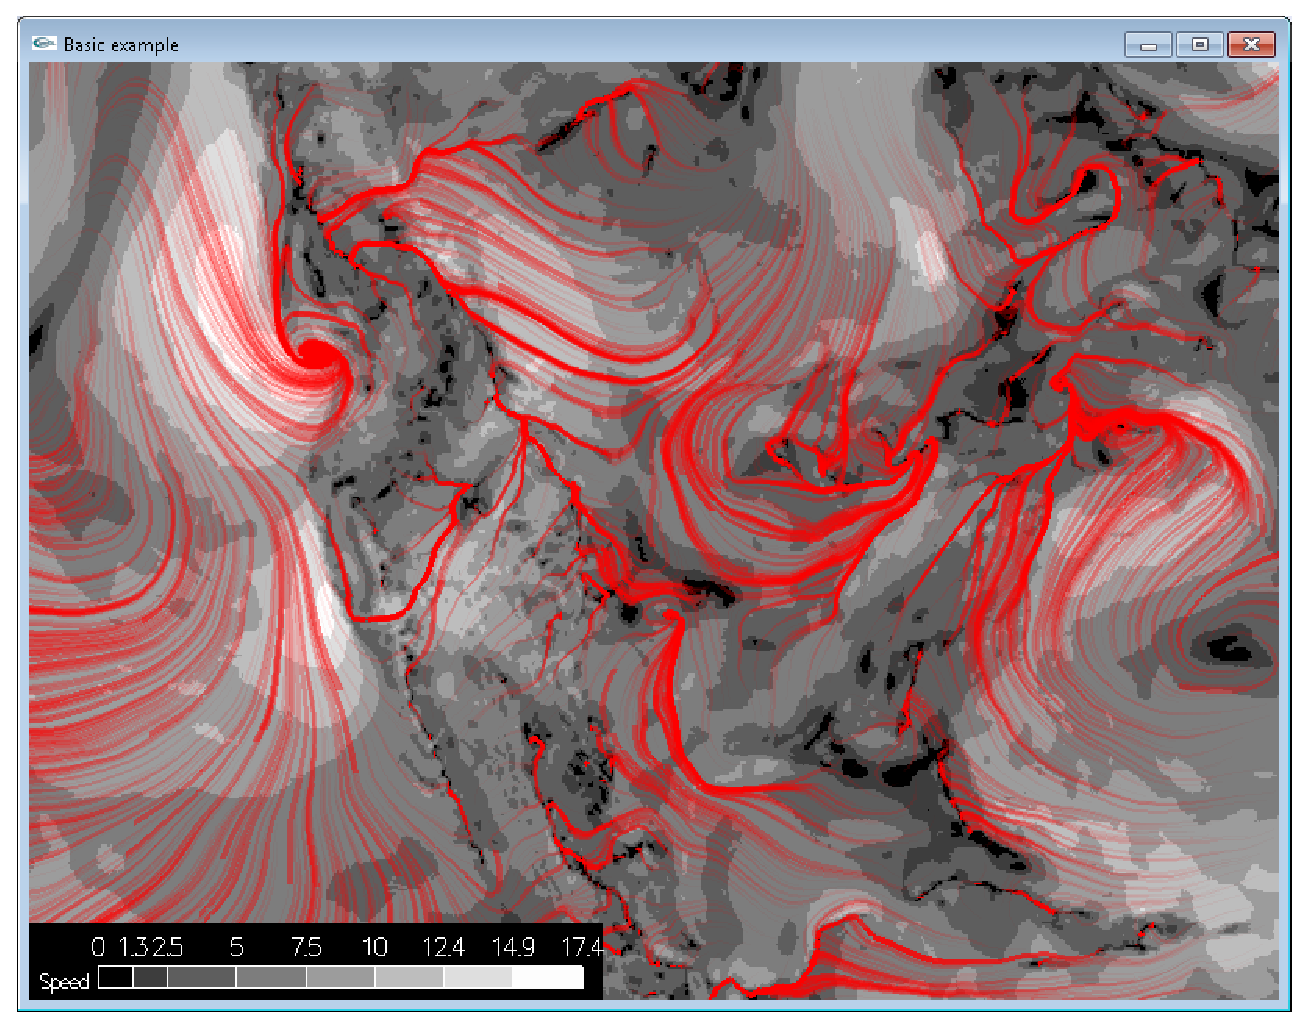
\includegraphics[height=1.2in]{images/basic_bw_red.eps}
   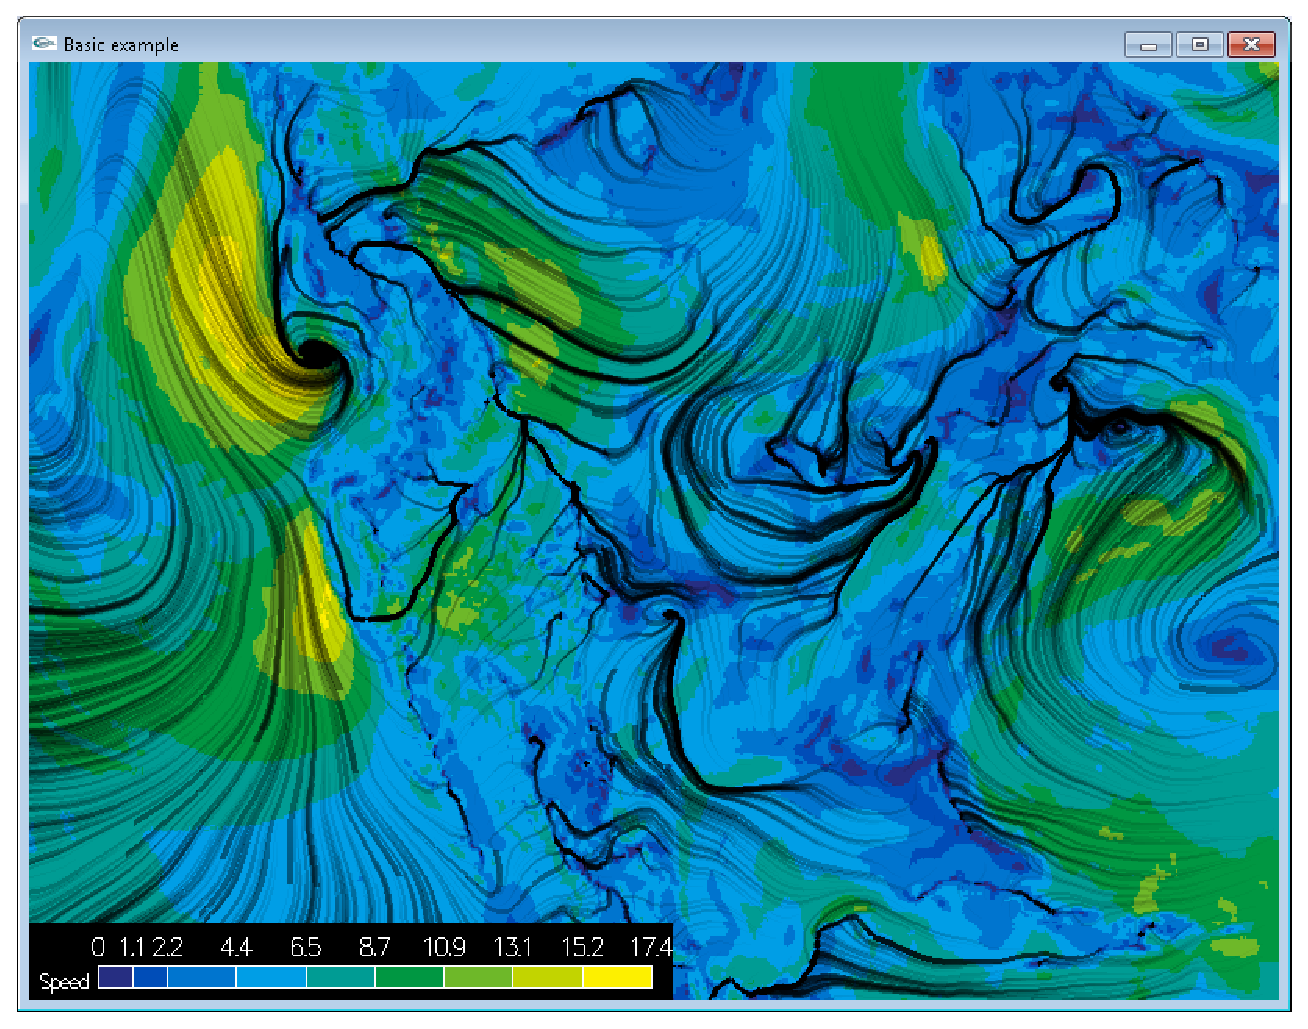
\includegraphics[height=1.2in]{images/basic_by_black.eps}
   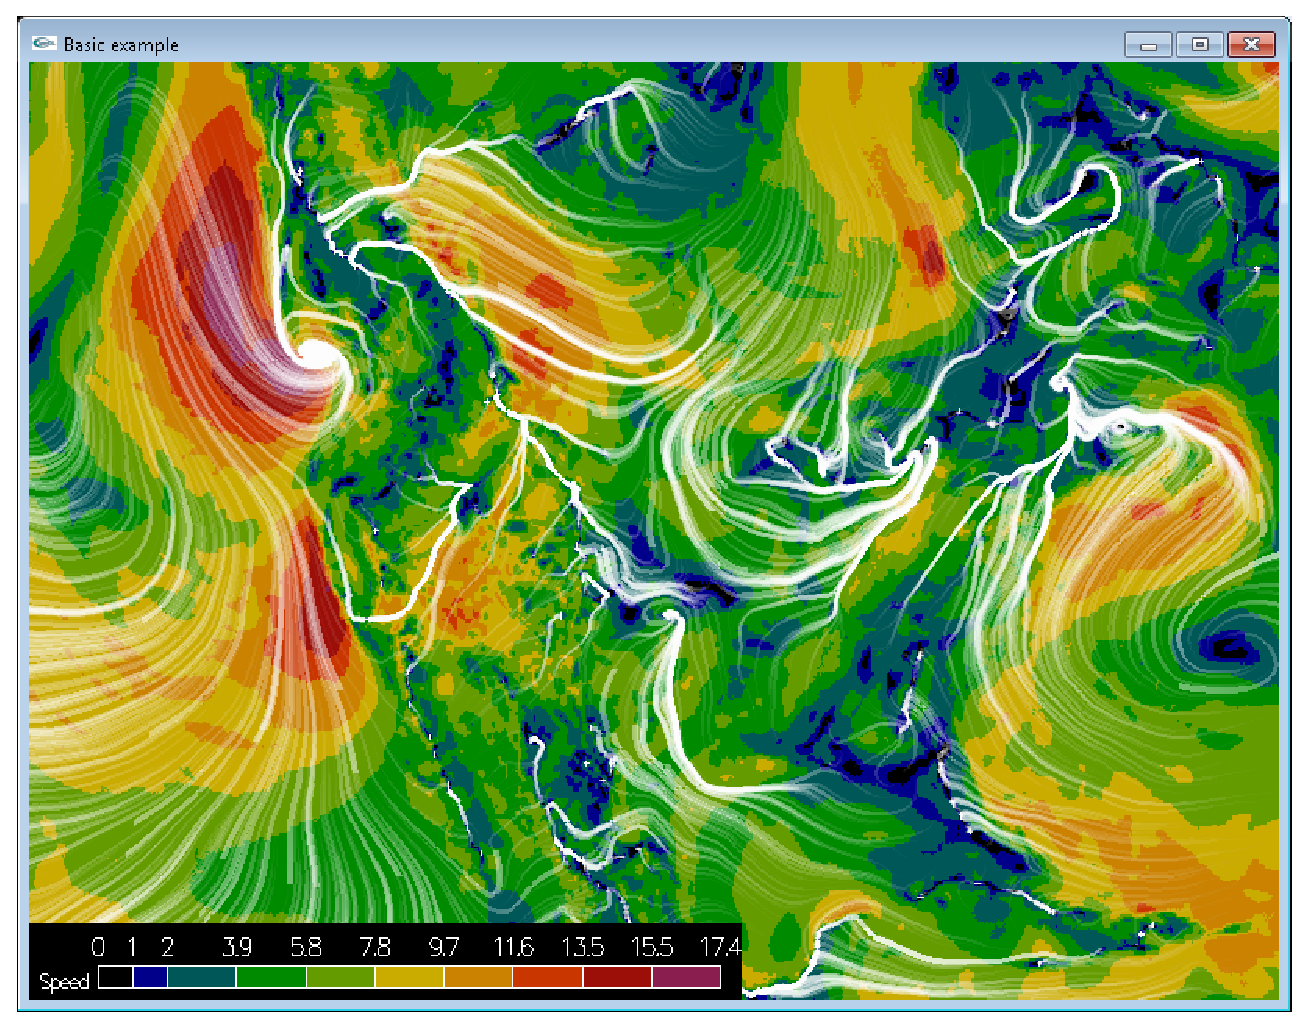
\includegraphics[height=1.2in]{images/basic_rainbow_white.eps}
    \caption{Three possible color combinations: red traces on a black-to-white scale, black traces on a blue-to-yellow scale, and white traces on a rainbow scale.}
   \label{fig:colors}
%\end{wrapfigure}
\end{figure}

I have colored my background according to the wind speed at each grid cell.  There are three choices for color scales of the background: black-to-white, blue-to-yellow, and rainbow.  First, this required finding the minimum and maximum wind speeds in the dataset.  Next, I created speed intervals for coloring according to the chosen color set. The intervals are evenly spaced between the minimum and maximum speed values, except for the first two intervals.  The first and second intervals are half the size of all other intervals; this was done so that slower winds could be distinguished from near zero winds more easily.  

The particle traces themselves are all colored one color -- either white, black, or red.  The ``older" end of a particle trace is thinner than the ``newer" end of the particle.  The particle trace is also more transparent (0.02 opacity) at the ``older" end than at the ``newer" end (0.45 opacity).  Therefore, the direction can be discerned by both the thickness and opacity.  The thickness of the particle trace is also increased slightly when the particle is moving faster, however this effect is not emphasized much in order to reduce visual clutter.

Right-clicking allows the user to choose a color scale for the background, choose a color for the particle traces, and toggle the legend which explains the background.

\textit{Comment on effects. E.g., how does gray scale change affect the presentation of direction in relation to the background value. Difficulties and possible solutions may also be mentioned.}

My three color scales for the background were carefully chosen.  First, the rainbow background came from searching the web for various visualizations of wind speeds and seeing that many used some variation of a rainbow scale.  Second, the blue-to-yellow was chosen because it does not include both red and green, which can be problematic for color blind people.  Third, the black-to-white scale was chosen because it is easy to understand since it only varies in lightness, as opposed to the others which may vary in lightness and saturation in addition to hue.  The three colors for the traces were chosen because they can easily contrast against at least one of the backgrounds.

\begin{figure}[htb]
%\begin{wrapfigure}{r}{0.4\textwidth}
   \centering
   
\includegraphics[height=1.1in]{images/inwardspiral.eps}
   
\includegraphics[height=1.1in]{images/outwardspiral.eps}
   
\includegraphics[height=1.1in]{images/front.eps}
    \caption{An inward spiral, an outward spiral, and a front.}
   \label{fig:features}
%\end{wrapfigure}
\end{figure}

I found that the red on the black-to-white background is easiest to interpret, even if it does not make for the ``prettiest" picture.  However, I feel it is easiest to find the areas with the fastest winds when using the blue-to-yellow background.  The rainbow background is perhaps best for discerning what wind speed interval a particular grid cell falls in, but it otherwise is cluttered looking.

The features can be easily found using all backgrounds with an appropriately contrasting color for the traces, but they seem to stand out most with red on black-to-white.  I played with the number of particles by increasing it until the various features were apparent, while also making sure that the particles didn't completely cover the background. 

\end{document}

